\chapter{新的基于几何构建的算法 (GBEM-LLS 和 GBEM-NLS) 及数值实验}
\label{cha:ouralg}

由于每一步涉及的都是小规模的易于求解的子问题, 相比于基于 SDP 松弛的算法, 
几何构建算法 (GB-LLS 和 GB-NLS) 非常快. 
然而, 已有的几何构建算法, 即便是最新的版本 \cite{Sit2009},
只能容忍数据中存在非常小的误差, 一般不超过 $0.01\%$, 
这使得该算法并不能很好地解决实际问题.
特别地, 即便是对于精确距离的情形, 当蛋白质中原子个数较多时 (多于几千),
舍入误差的累积 (error accumulation) 都会导致最终的结构完全偏离正确结果,
对于一般有误差的情形, 结果只会更糟.

这就是我们开始这项研究的最初的动机, 我们想要分析误差形成的原因,
并发展一些新的技术来客服误差累积的困难.
我们最终提出的算法可以看作是对已有几何构建算法的改进.
而另一个看待我们的算法的角度是, 
总的来看, 新的算法致力于求解一个误差函数极小问题, 我们的目标是求全局极小值点,
而问题却有特别多的局部极小值点, 所以我们要通过几何构建算法来去找一个好的初值点.
而从每一步来看, 我们解的是只跟很少项有关的子问题,
这也是借助了几何构建的思想.
总而言之, 为了使新算法快速而精确, 几何构建和优化过程同样地重要.

本章的结构如下. 
在 \ref{sec:ErrImportant} 中, 我们讨论为什么数值误差如此重要.
在 \ref{sec:ErrAnalysis} 中, 我们分析已有算法中, 误差的来源.
在 \ref{sec:CompOrder} 中, 我们给出一个有效的计算顺序策略.
在 \ref{sec:opt} 中, 我们讨论优化的子问题及其求解方法.
在 \ref{sec:framework} 中, 我们总结前述讨论, 给出算法的总体框架.
在 \ref{sec:NumResult} 中, 我们给出大量的数值实验结果, 并加以分析.
\ref{sec:summary} 是本章的总结.
最后, 在 \ref{sec:CodeWrite} 和 \ref{sec:ErrExample} 中, 
我们以附录的形式分别讨论算法的几个关键代码实现, 以及给出一个舍入误差累积的例子.

\section{为何数值误差很重要~?}
\label{sec:ErrImportant}

计算误差的累积是几何构建算法中的很严重的问题 \cite{Wu2006,Wu2008}, 
这在我们自己的数值实验中也得到了观察.
图 \ref{fig:OriginalOrder} 给出了一组典型的 RMSD\footnote{详细定义会在 \ref{sec:NumResult} 中给出, 在此可理解为所有点坐标的平均误差.} 结果,
这是将 GB-LLS 应用到计算蛋白质 1MQQ 得到的, 其中假设距离是精确的.
从理论上讲, 这个算法能够保证得到一个精确的蛋白质结构 \cite{Sit2009}. 
但是在实际计算中, 尽管 RMSD 在最开始的几百步非常好, 
可是它随着迭代的进行上升地非常快,
最后在差不多3500步的时候就完全错了.
这个例子表明, 算法 GB-LLS 在理论和数值表现上存在一个不可忽视的鸿沟,
这促使我们设计更加鲁棒 (robust) 的算法来解决这一问题.

\begin{figure}[htbp!]
  \centering
  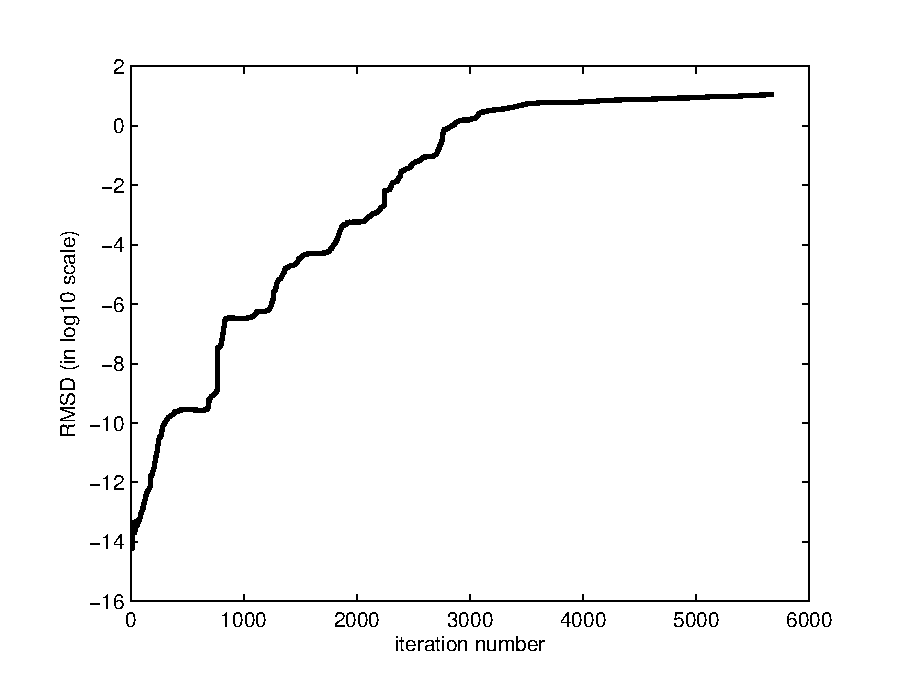
\includegraphics[width=0.5\textwidth]{OriginalOrder.eps}\\
  \caption{将 GB-LLS 应用到计算蛋白质 1MQQ (5681个原子) 的 RMSD 结果 (距离是精确的, 距离阈值设为 6\AA). 结果经过了 $log10$ 函数换算, 表示的是 RMSD 的量级.}
  \label{fig:OriginalOrder}
\end{figure}


\section{已有几何构建算法的误差累积分析}
\label{sec:ErrAnalysis}
在这里我们考虑一种简单的情形, 也就是给定的距离都是精确的,
并且使用线性最小二乘来确定未知点. 
也就是说, 我们分析算法 GB-LLS 的一个迭代步.

假设点 $j$ 是要定位的未知点, 已知 $l$ 个到已知点 $1,2,\ldots,l$ 的距离. 
假设真实的坐标\footnote{我们可以固定最初确定的4个点为锚点, 剩下的点就可以用绝对坐标表示了.}
是 $\widehat{x}_i$, 而计算的坐标是 $x_i$, 
我们记该步之前点 $i$ 的定位误差为 $\delta x_i=x_i-\widehat{x}_i$,
并且进一步假设这些误差在同一个量级, 记为 $\delta x_i=O(\delta x)$.

我们需要求解最小二乘 $\min_{x_j} \|Ax_j-b\|$, 其中
\be A = 2[(x_{i+1}-x_i)^T], b=[(\|x_{i+1}\|^2-\|x_i\|^2)-(d_{i+1,j}^2-d_{ij}^2)],~i=1,2,\ldots,l-1.\ee
从而, 我们有
\begin{align}
  \|x_{i+1}\|^2-\|x_i\|^2 & = \|\widehat{x}_{i+1}+\delta x_{i+1}\|^2-\|\widehat{x}_i+\delta x_i\|^2    \\
  & = \|\widehat{x}_{i+1}\|^2-\|\widehat{x}_i\|^2 + 2\widehat{x}_{i+1}\delta x_{i+1} - 2\widehat{x}_i\delta x_i + \delta x_{i+1}^2-\delta x_i^2.
\end{align}
所以, $A=\widehat{A}+O(\delta x),~~b=\widehat{b}+O(\delta x)$, 进一步地, 
\begin{align}
  \|Ax_j-b\| & =\|(\widehat{A}+\delta A)(\widehat{x}_j+\delta x_j)-(\widehat{b} + \delta b)\| \\
  & =\|\widehat{A} \delta x_j + O(\delta x)\|.
\end{align}
从以上分析我们可以得出, 每一个构建步的误差主要来自三个方面:
\begin{enumerate}
  \item 从之前的计算中遗传下来的误差, 这些误差隐含在 $A$ 和 $b$ 中, 是构建步的主要误差来源.
  \item 由坏条件数 (ill-conditional) 的 $A$ 引起的计算误差, 这只会在很少的迭代步中占主导因素, 但有时会引起大的误差.
  \item 由有限精度计算带来的舍入误差.
\end{enumerate}

在计算中, 上述几种误差都是掺杂在一起的, 互相影响.
舍入误差我们无能为力, 所以我们的目标是设计算法避免坏条件数的 $A$,
并且尽量使之前的定位更加精确, 从而减小 $A$ 和 $b$ 中带来的误差.


\section{计算顺序: 选择新加入点的策略}
\label{sec:CompOrder}

\subsection{引言}
注意到几何构建算法是一个一个地确定所有点的坐标, 
并且依靠已知点的坐标和未知点到已知点的距离来决定未知点,
所以, 很显然, 先确定的点的精度将会对后续定位的点的精度产生重大影响.
这就是我们要考虑的计算顺序的问题.

在已有的几何构建算法中, 他们利用的是 PDB 文件\footnote{我们将在数值实验部分 \ref{sec:NumResult} 详细解释.}
中原子的默认顺序.
所以, 他们实际上隐式地利用了蛋白质的结构信息.
这种结构信息是有用的, 但在实际问题中是很难知道的, 
一般来说我们知道的只有距离信息 \cite{Dong2002}.
所以, 在本文中我们试图设计一种仅仅利用距离信息的规则,
这样会比较实际.

\subsection{新规则的定义和讨论}
基于以上分析和讨论, 我们提出利用以下两种信息来选择点 $j$ 作为未知点.
\begin{itemize}
  \item (结构信息)%: the largest number of known distances \\
  ~记 $\mathcal{Y}$ 是已知点的集合, $\mathcal{N} = \{1,2,\ldots,n\}\backslash \mathcal{Y}$ 是未被确定的点的结合, 我们定义
  \be p(i) = \sharp \{d_{ik}\neq 0: k\in \mathcal{Y}\}, ~~对所有的~i\in \mathcal{N}, \label{rule1} \ee
  并进一步定义
  \be \mathcal{I} = \{i: p(i) = \max_{k\in \mathcal{N}} ~p(k)\}, \label{rule2}\ee
  其中 $p(i)$ 是未知点 $i$ 到已经确定的点中已知距离的数目, $\mathcal{I}$ 是拥有最多的已知距离的未知点的集合.
  \item (距离信息)%: closest to the determined points \\
  ~我们选择点 $j$ 满足
  \be j = \arg\min_{i\in \mathcal{I}} \sum_{k\in \mathcal{Y}} d_{ik}, \label{rule3}\ee
  它是集合 $\mathcal{I}$ 中到已知点距离``最近''的点, 这里最近的意义是已知距离的和.
\end{itemize}

直观上看, 我们选择已知最多数目的距离, 并且离已知点最近的点.
在很多时候, 都会有多个点满足第一个规则, 所以我们需要第二个规则,
从而避免使算法不稳定或不可预测.

这个计算顺序的好处包括但不限于以下几个方面:
\begin{enumerate}
  \item 摇摆现象被消除了. 在已有的几何构建算法中, 我们经常观察到构建步会进行到离已知点整体比较远的地方, 再迭代回来. 在新的规则下, 这种来回摇摆的现象消失了.
  \item 作为前一点的结果是, 在往更远处迭代的时候, 通常已知点都是聚成团的, 其附近的点都已被确定, 这样在计算新的未知点的时候, 将会有更多的距离被用到. 更多的距离对提升算法的精准度和稳定性都是有帮助的.
  \item 整个算法更加稳定. 这里稳定的意义是, 这个规则下得到的系数矩阵 $A$ 的条件数通常都比较小, 求解线性最小二乘子问题的数值稳定性更好. 这一点在数值实验中得到了证实.
\end{enumerate}

\subsection{一个构造的简单例子}
在本节中, 我们构造了一个简单的二维例子, 如图 \ref{fig:CompOrder} 所示,
来说明计算顺序的重要性.
在这个例子中, 我们有6个点, 他们的序号和位置如图所示,
其中由点1和点2所决定的直线是水平的.
点之间已知的距离由实线表示.

\begin{figure}[htp]
  \centering
  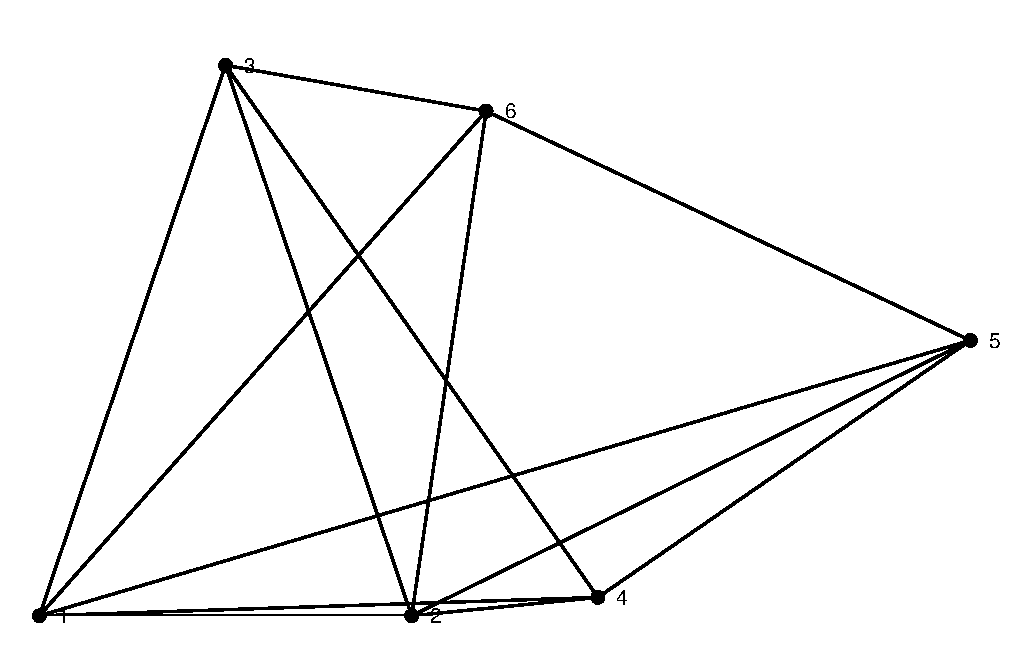
\includegraphics[width=0.5\textwidth]{CompOrder.eps}\\
  \caption{一个简单的例子, 用以表明计算顺序的重要性}
  \label{fig:CompOrder}
\end{figure}

我们应用原始的 GB-LLS 来求解该问题. 
点 1,2,3 作为基准点首先被定位, 接着点 4,5,6 按次序一个一个被确定.
这个过程看起来非常完美, 但却暗含潜在的风险.
我们假设 $d_{34}$ 的测量不准确, 从而使得点4的定位在很小的扰动下到了水平线之下.
如果我们仅仅看前四个点, 结果还是可以接受的, 因为仅仅是第四个点有很小的误差. 
接着我们根据点1,2,4的位置定位点5,
它也将会定位在水平线之下, 从而产生非常大的误差.
最后, 点6也不能很好地被定位.
从代数上来看, 点4的小扰动使得点5的定位产生大的误差的原因是,
点 1,2,4 几乎在同一条直线上, 从而形成的系数矩阵 $A$ 是坏条件数的.

现在我们来看, 这种数值上的风险在我们的规则下是如何消失的.
最开始的两步跟原算法是一致的, 不同的是我们会先于点5确定点6,
因为他们都已知到确定点\pozhe 1,2,3,4 的三个距离, 但点6离它们(总距离)更近.
在点6被正确地定位后, 点5也就可以被很好地定位了,
因为此时我们可以利用四个距离, 而点1,2,4,6 可以形成一组稳定的基,
得到一个小条件数的 $A$.
这个人造的例子表明了我们的策略确实是有效的, 
在真实的蛋白质数据上的测试结果将在 \ref{sec:NumResult} 中给出.


\section{误差函数极小}
\label{sec:opt}
\subsection{子问题}
我们先介绍图论中诱导子图的概念. 
$G=(V,E)$ 是一个图, 其中 $V$ 是顶点集, $E$ 是边集.
$V'\subseteq V$ 是顶点集的一个子集, 
那么 $G(V')=(V',E')$ 就称为图 $G$ 的诱导子图, 
其中 $E'=\{(i,j)\in E: i\in V', j\in V'\}$.

在每一个构建步之后, 我们提出增加一个在子图 $G(j\cup N(j))$ 上的优化步, 
其中 $N(j)=\{k: d_{jk}\neq 0\}$ 是点 $j$ 的邻接点的集合. 
也就是说, 我们进一步求解以下子问题
\be \min  f(x_{j\cup N(j)}), \label{prob:sub}\ee
其中 $f(\cdot)$ 是定义在诱导子图 $G(j\cup N(j))$ 上的误差函数, 
未知距离\footnote{因为 $x_i$ 是要求解的坐标, 我们把 $\|x_i-x_j\|$ 称作未知距离.}到已知距离的偏差在边集 $E'$ 上被加和. 
%We choose $f(\cdot)$ as $Stress(\cdot)$ in (\ref{eqn:stress}) with $\omega_{ij}=1$ in this paper.

%\subsubsection{Comments and further discussion on error function}
注意到问题 (\ref{prob:sub}) 中的目标函数
与我们最终要求解的优化问题有着完全相同的形式,
但只包含集合 $j\cup N(j)$ 中点内部的距离.
由于实际问题中, 距离是稀疏而局部的 (sparse and local),
我们得到的是小规模的问题 (通常不多于几十个变量),
同时构建步可以提供一个高质量的初始点,
所以子问题 (\ref{prob:sub}) 通常可以在很少的迭代步之内被高精度地求解.
所以, 由增加的优化步所带来的计算量并不大.

从另一个角度来看, 考虑到距离信息的使用,
优化子问题可以看作线性最小二乘与非线性最小二乘的折衷.
就像我们之前提到的, GB-LLS 仅仅使用 $l$ 个距离\pozhe 太少,
GB-NLS 不但利用了已知的距离, 还利用了计算的距离\pozhe 太多, 
而我们在这两种极端方法中找了一个有效的折衷\pozhe 我们使用了
相关的全部距离, 但不使用计算出来的距离.
这样做的好处是多方面的.
我们既保留了 GB-NLS 的优点\pozhe 稳定性以及根据新加入的点和距离调整已知点的能力,
又克服了它的缺点, 避免了误差通过计算的距离而累积.
而且, GB-NLS 的关键步是使用矩阵分解算法,
是在变换后的距离矩阵上做运算,
而我们做的是误差函数极小化, 
更加符合原问题的本质\pozhe 距离尽可能地被满足.

\subsection{求解算法}
我们可以计算 $Stress$ 的导数如下所示,
\be \frac{\partial Stress}{\partial x_i}=2\sum_{j\in N(i)} \Big(1-\frac{d_{ij}}{\|x_i-x_j\|}\Big)(x_i-x_j), \label{gradient}\ee
其中 $N(i)$ 是 $i$ 的邻接点集合.

在本文中, 我们主要利用带 Barzilai-Borwein (BB) 步长 \cite{BB1988} 
的梯度法来求解 (\ref{prob:sub}). 
如果 BB 步连续 $M$ 次没有改进, 
我们也结合 Armijo 回溯线搜索 (backtracking line search) 来保证收敛性,
请参考 \cite{Armijo1966,Sun2006}.

\textbf{Armijo 回溯线搜索} ~令 $\alpha = \delta\beta^i$, 
其中 $\delta>0$ 是初始步长, 
$i$ 是满足下式的最小的非负整数
\be f(x)-f(x+\delta\beta^id)\geq -b\delta\beta^i d^T\nabla f(x), \ee
其中, $b\in (0,1)$ 是一个参数, $d$ 是搜索方向.

在迭代中, 
$\delta^k=\frac{\|s^{k-1}\|^2}{{s^{k-1}}^Ty^{k-1}}$ 是第$k$步的长 BB 步长, 
其中 $s^k=x^k-x^{k-1}$, $y^{k-1}=g^k-g^{k-1}$, 而 $x^k$ 是迭代点,
$g^k$ 是梯度. 
迭代格式如下
\be x^{k+1} = x^k + \alpha^kd^k.\ee

%We also apply the following nonmonotone line search technique to make our algorithm have to ability to escape from some not so good local minimizers.

\section{算法总框架}
\label{sec:framework}
在本节中, 我们对前几节的讨论作一个总结,
给出我们的算法 GBEM
的总体框架.
%
%\begin{algorithm}[H]
%\SetKwInOut{Input}{input}\SetKwInOut{Output}{output}
%\Input{A symmetric distance matrix $D$} %to specify part of the pairwise distances}
%\Output{index set of determined points and coordinate matrix $X$}
%%\vskip1mm
%Find a maximal clique that are not in the same plane\;
%Use Matrix Decomposition Method to determine these points\;
%%Repeat:
%
%\While{not all the points are determined}{
%Find point $j$ according to \reff{rule1}, \reff{rule2} and \reff{rule3}\;
%\eIf{$l=p(j)\geq 4 ~\&~ N(j) \textrm{ not in the same plane}$}
%{Determine $x_j$ by linear \reff{LLS} or nonlinear least square \reff{NLS}\;
%Adjust the locations of points $j\cup N(j)$ by solving \reff{prob:sub}.
%}
%{No more point can be uniquely determined\;
%Return the determined index set and coordinates, stop.}
%}
%\caption{Enhanced Geometric Buildup for sparse noisy anchor-free Distance Geometry Problem}
%\end{algorithm}

\begin{Alg} (GBEM \footnote{Geometric Buildup-based Error Minimization (简记为 GBEM), to solve sparse, noisy and anchor-free distance geometry problem.})
  \begin{adjustwidth}{1cm}{0cm}
    \begin{enumerate}[步1.]
      \item 找一个不是所有点都在同一个平面上的极大团, 利用矩阵分解算法 (\ref{sec:MatDcomp}) 确定这些点的坐标. 令 $\mathcal{T}=$ \{确定点的指标\}.
      \item 根据 (\ref{rule1}), (\ref{rule2}) 及 (\ref{rule3}) 找到指标 $j$. 如果 $l=p(j)\geq 4$, 且 $N(j)$ 中的点不都在同一个平面上, 转步3, 否则转步5.
      \item 用线性最小二乘 (\ref{LLS}) 或非线性最小二乘 (\ref{NLS}) 计算坐标 $x_j$, 并求解子问题 (\ref{prob:sub}), 调整 $x_{j\cup N(j)}$. 令 $\mathcal{T}=\mathcal{T}\cup \{j\}$.
      \item 如果所有点都已确定, 转步5, 否则转步2.
      \item 求解定义在 $\mathcal{T}$ 上的问题 (\ref{prob:error}), 停止.
    \end{enumerate}
  \end{adjustwidth}
%\caption{基于几何构建的误差极小算法 GBEM, 用来求解稀疏的带误差距离的, 无锚节点距离几何问题.}
  \label{alg:EGB}
\end{Alg}
根据步3中计算方法的不同, 我们把新提出的算法分别叫做
GBEM-LLS 和 GBEM-NLS.

%
%\subsection{Subspace point of view}
%Subspace is not a new concept but somehow a new aspect to view an algorithm \cite{Yuan2007}, and also useful philosophy to design algorithm to solve large-scale problems. We now focus the optimization problems solved in Algorithm \ref{alg:EGB} and explain this algorithm in subspace fashion.
%
%Our final task is to solve \reff{prob:error} (Step 5), which is an optimization problem with $n$ points thus totally $n\times  d$ variables. Instead of solving this difficult problem directly, we actually choose to iteratively minimize this function restricted at subspace $x_{j\cup N(j)}$ (Step 3), which is much easier to solve.
%
%\subsection{Convergence}
%The convergence of Algorithm \ref{alg:EGB} to a local minimizer is guaranteed by the standard theory of gradient method with Barzilai-Borwein step size \cite{BB1988,Sun2006}. However, as we have stated before, this local convergence is of little meaning in practice. On the other hand, the convergence to global solution is not easy to prove (actually, we believe there exist counterexamples, but this kind of example is meaningless for real applications, we do not waste our time to do that). Numerical results in next section will show that our algorithm can converge to global solution or very close to optimal solution in many instances.

\section{数值实验}
\label{sec:NumResult}
关于距离几何问题, 我们没有找到任何公开的测试数据集.
即使对于蛋白质折叠, 不同的文章使用的都是不同方式构造的模拟数据.
例如, 在 DAFGL \cite{Biswas2008} 中, 
作者使用了部分距离小于 6\AA ~(1\AA ~= $10^{-10}$m)~ 的上下界数据.
而在改进的 DISCO \cite{Fang2013} 中, 
20\% 的距离小于 6\AA 的带误差的数据被使用,
但作者结合了从化学知识推断出的其他距离信息.
所以, 想要把我们的算法跟已有的算法做一个直接的对比并不容易,
因为问题的设定并不完全相同, 而模拟数据的误差又是随机产生的.
在本文中, 我们将我们的算法跟已有的最新版本的几何构建算法 \cite{Sit2009} 作对比, 
尤其是展示新算法处理大误差数据的能力.

我们在 \ref{sec:ProbSet} 中介绍怎样构造测试数据集, 用来模拟真实的蛋白质数据.
在 \ref{sec:result} 中, 我们展示详细的数值结果, 
并且基于数值结果进行讨论分析, 给出一些结论.

\subsection{问题设定}
\label{sec:ProbSet}
我们先从蛋白质数据银行 (Protein Data Bank\footnote{\url{http://www.pdb.org}}, 
简称 PDB) \cite{Berman2000} 下载真实的蛋白质结构数据.
PDB 是一个由实验确定的三维蛋白质结构数据库, 
它包含蛋白质中的三维生物大分子结构数据.
根据 PDB 文件中原子的坐标, 我们使用圆盘图模型 (disk graph model) 来构造距离矩阵,
也就是说, 我们假设距离 $d_{ij}$ 是已知的, 
如果该距离小于或等于实现给定的距离阈值 
(cutoff, 通常为 5\AA ~或 6\AA, 其中 6\AA ~差不多是核磁共振技术
能够测量的两个原子之间的最大距离 \cite{Biswas2008}). 
通过这种方式, 我们模拟, 由于生物技术的限制,
只有小于一定阈值的距离才能够被测量这一真实情况.

在实际应用中, 测量到的数据通常都带有误差,
我们也在实验数据中通过添加正太分布或者均匀分布的乘性误差来模拟这一情况.
我们令测量到的距离 $d_{ij}$ 为
\be d_{ij} = \bar{d}_{ij}(1+\delta_{ij}*nl), \label{dij} \ee
其中, $\bar{d}_{ij}=\|\bar{x}_i-\bar{x}_j\|$ 是原子 $i$ 到原子 $j$ 之间的真实距离,
$\delta_{ij}$ 是一个遵从事先给定的分布的随机数.
例如, \cite{Biswas2008} 使用了标准正太分布 $\delta_{ij} \sim N(0,1)$,
而 \cite{Sit2009} 则使用了均匀分布 $\delta_{ij} \sim U[-1,1]$. 
我们在本文中汇报正态分布误差的结果, 
而略过在均匀分布上的结果, 对于我们的算法结果没有明显差别.
在 (\ref{dij}) 中,  $nl$ 是我们预先设定的误差水平,
在本文中等于 $1\%$, $5\%$, 或 $10\%$,
分别代表较小, 中等和较大的误差水平.

%\newcolumntype{R}{>{\flushright\arraybackslash}X}
%\renewcommand\arraystretch{0.85}
\setlength{\tabcolsep}{11.5pt}
\begin{table}[!htbp]
  \centering
  \footnotesize{
    \caption{测试问题信息汇总}
    \begin{tabular}{lrcccccccc}
      \toprule
      &  &  \multicolumn{4}{c}{cutoff = 5\AA} & \multicolumn{4}{c}{cutoff = 6\AA} \\
      \cmidrule(r){3-6}\cmidrule(r){7-10}
      \hd{ID}& \hd{Num} &  & \multicolumn{3}{c}{degree} &  & \multicolumn{3}{c}{degree}\\
      \cmidrule(r){4-6} \cmidrule(r){8-10}
      & & \hd{per} & max & min & avr &\hd{per} & max & min & avr \\
      \midrule
      1PTQ &  402 & 5.46 & 38 & 4 & 21.9 & 8.79 & 61 &  6& 35.3  \\
      1HOE &  558 & 4.05 & 38 & 6 & 22.6 & 6.55 & 65 & 11& 36.5  \\
      1LFB &  641 & 3.40 & 40 & 5 & 21.8 & 5.57 & 59 &  8& 35.7  \\
      1PHT &  811 & 3.35 & 48 & 5 & 27.1 & 5.37 & 75 &  7& 43.5  \\
      1POA &  914 & 2.51 & 39 & 4 & 22.9 & 4.07 & 67 &  8& 37.2  \\
      1AX8 & 1003 & 2.30 & 39 & 5 & 23.0 & 3.74 & 59 &  7& 37.5  \\
      4MBA & 1083 & 2.17 & 39 & 5 & 23.5 & 3.56 & 60 &  5& 38.5  \\
      1F39 & 1534 & 1.47 & 40 & 5 & 22.6 & 2.43 & 62 &  7& 37.2  \\
      1RGS & 2015 & 1.12 & 41 & 3 & 22.6 & 1.87 & 66 &  4& 37.7  \\
      1KDH & 2846 & 0.83 & 43 & 4 & 23.6 & 1.36 & 64 &  5& 38.8  \\
      1BPM & 3671 & 0.66 & 42 & 3 & 24.4 & 1.12 & 64 &  4& 40.9  \\
      1RHJ & 3740 & 0.65 & 40 & 4 & 24.4 & 1.10 & 61 &  5& 41.2  \\
      1HQQ & 3944 & 0.60 & 40 & 3 & 23.7 & 1.00 & 64 &  5& 39.5  \\
      1TOA & 4292 & 0.56 & 39 & 3 & 24.0 & 0.94 & 62 &  4& 40.1  \\
      1MQQ & 5681 & 0.44 & 44 & 5 & 25.2 & 0.75 & 66 &  7& 42.4  \\
      1HMV & 7398 & 0.32 & 42 & 3 & 23.3 & 0.52 & 67 &  4& 38.7  \\
      1I7W & 8629 & 0.29 & 48 & 3 & 24.7 & 0.47 & 73 &  5& 40.9  \\
      \toprule
    \end{tabular}\\[-3mm]
    \label{table:probinfo}
    \begin{flushleft}
      *ID---PDB 中蛋白质的ID, Num---蛋白质中原子的数目, per---已知的距离占所有的两两距离的百分比, degree---所有点的最大/最小/平均度
    \end{flushleft}
  }
\end{table}
我们用 GBEM-LLS 和 GBEM-NLS 计算文章 \cite{Biswas2008} 和 \cite{Sit2009}
用到的所有 17 个蛋白质, 其原子个数从 402 到 8629 不等. 
我们将测试问题的信息在表 \ref{table:probinfo} 汇总. 
表的第一列是 PDB ID, 它是蛋白质在 PDB 中独一无二的标识. 
第二列是每一个蛋白质中原子的个数, 也就是我们问题中点的个数. 
在第三列, 我们仿照 \cite{Biswas2008} 给出距离矩阵的稀疏度, 
它是已知的距离占所有的两两距离的百分比,
更稀疏的问题意味着我们知道``更少''的距离, 在一定程度上反映了问题的难度.
但是, 我们并不认为这是一个描述问题难度的很准确的标准.
比如, 假设我们将一个图复制 9 份, 并且增加少量必要的距离使得图形成一个刚性结构,
这样, 已知的距离差不多是 10 倍多 (呈线性增加), 
而总的两两距离的数目是平方量级的, 也就是说, 差不多 100 倍多, 
所以问题的稀疏度显著地增加了, 但问题的难度, 
除了存储和计算时间的考虑, 并没有显著地增加.
这个例子表明, 这个标准跟我们的直觉 \pozhe ``越稀疏的问题, 难度会显著增加''
并不是很吻合.
更准确地说, 当问题中点的数量差不多时, 稀疏度才是一个有意义的衡量问题难度的标准.
所以, 在本文中, 我们提出结合所有点的度 (degree) 的信息来说明问题的难度.
在 4--6 列中, 我们给出问题的最大, 最小和平均度.
我们将会看到, 度信息能更好地反映问题的难度, 尤其是对几何构建类的算法.
最后四列跟 3--6列是类似的, 不过把距离阈值从 5\AA ~增加到 6\AA,
也就是假设知道更多的距离信息.

我们的程序完全是用 Matlab 写的.
程序中最耗时的部分是循环计算梯度值, 
而这部分可以用 C 语言写, 并编译成 MEX 文件来加速,
但我们并没有这么做.
本节中所有的实验结果都是在 Dell 个人电脑上运行的,
其 CPU 为 2.83 GHz, RAM 为 4.00 GB, 
使用的程序版本为 Matlab R2013b, 8.2版.

\subsection{实验结果比较标准}
\label{sec:result}
我们将算法 GBEM-LLS 和 GBEM-NLS 应用到距离矩阵上.
注意, 我们的算法需要的唯一信息就是距离,
点的正确坐标仅仅是用来检验定位的精确度 (accuracy),
它是由如下定义的均方根偏差 (Rooted Mean Squared Deviation, 缩写为 RMSD\footnote{我们在后文还会见到其他相关的标准, 如函数值等, 但我们认为 RMSD 是衡量定位精度的最可信的标准. 在本文中, 我们所称的定位精度都是指 RMSD 值的大小.}) 来衡量的:
\be RMSD(X,Y) = \min_{Q,T}\{ \|Y-XQ-T\|_{F}/\sqrt{n}: \Tran{Q}Q=I\}, \ee
其中, $X\in \Real^{n\times 3}$ 和 $Y\in \Real^{n\times 3}$ 
分别是计算的和真实的坐标矩阵, 
$T$ 是平移向量, $Q$ 是正交矩阵.
粗略地讲, 我们通过刚性变换移动 $X$, 使其与 $Y$ 尽可能地吻合,
而 RMSD 衡量的就是移动后最小的偏差. 
需要特别注意的是, RMSD 仅能用来事后检验算法的表现,
并不能用来当作算法终止准则 (stopping criterion), 
因为它的计算要用到真实的坐标矩阵 $Y$,
而这是实际应用中是未知的.
事实上, 各种算法都是使用跟误差函数相关的量作为停机准则,
比如函数值, 或梯度模. 
其中文章 \cite{Biswas2008} 使用的一个终止准则定义如下:
\be LDME = \Big(\frac{1}{|E|} \sum_{(i,j)\in E}\big(\|x_i-x_j\|-d_{ij}\big)^2\Big)^{1/2}. \ee
但正如作者在文中指出的, 
LDME (Local Distance Matrix Error) 虽然在计算上更实际, 
但并不是一个很可靠的标准, 
更小的 LDME 值并不一定意味着更精确的定位 (尽管在很多例子中成立).
所以, 在前几个主要结果中, 我们没有列出函数值的相关结果, 
尽管我们使用误差函数值和梯度模作为优化步中的终止准则.

\subsection{计算顺序的影响}
\setlength{\tabcolsep}{5.5pt}
\begin{table}[!htbp]
  \centering
  \footnotesize{
    \caption{精确距离情形下的 RMSD (\AA) 结果}
    \begin{tabular}{lrcccccccc}
      \toprule
      &  & \multicolumn{4}{c}{cutoff = 5\AA}
      & \multicolumn{4}{c}{cutoff = 6\AA} \\
      \cmidrule(r){3-6} \cmidrule(r){7-10}
      \hd{ID} & \hd{Num} & \multicolumn{2}{c}{LLS} & \multicolumn{2}{c}{NLS} & \multicolumn{2}{c}{LLS} & \multicolumn{2}{c}{NLS} \\
      \cmidrule(r){3-4} \cmidrule(r){5-6} \cmidrule(r){7-8} \cmidrule(r){9-10}
      & & \hd{GB} & \hd{GBnew} & \hd{GB} & \hd{GBnew} & \hd{GB} & \hd{GBnew} & \hd{GB} & \hd{GBnew} \\
      \midrule
      1PTQ &  402 & 1.4e$+$00 & 6.5e$-$13 & 5.5e$-$14 & 5.1e$-$14 & 2.6e$-$09 & 2.8e$-$14 & 5.0e$-$14& 2.9e$-$14  \\
      1HOE &  558 & 5.8e$-$02 & 3.0e$-$13 & 1.6e$-$13 & 2.4e$-$14 & 3.1e$-$09 & 3.8e$-$14 & 2.7e$-$13& 2.0e$-$14  \\
      1LFB &  641 & 2.0e$-$02 & 9.3e$-$14 & 9.5e$-$14 & 3.1e$-$14 & 2.1e$-$10 & 4.6e$-$14 & 5.5e$-$14& 2.1e$-$14  \\
      1PHT &  811 & 1.2e$+$01 & 2.0e$-$12 & 1.1e$-$13 & 6.3e$-$14 & 8.2e$-$09 & 9.3e$-$14 & 1.8e$-$13& 5.7e$-$14  \\
      1POA &  914 & 6.6e$+$00 & 8.2e$-$13 & 3.2e$-$13 & 7.4e$-$14 & 1.9e$-$09 & 2.8e$-$13 & 1.5e$-$13& 4.7e$-$14  \\
      1AX8 & 1003 & 5.2e$+$00 & 1.1e$-$11 & 4.0e$-$13 & 3.3e$-$14 & 1.8e$-$05 & 5.4e$-$14 & 4.6e$-$12& 3.0e$-$14  \\
      4MBA & 1083 & 4.9e$+$00 & 3.6e$-$12 & 1.8e$-$13 & 8.2e$-$14 & 3.8e$-$06 & 1.2e$-$13 & 2.6e$-$13& 6.9e$-$14  \\
      1F39 & 1534 & 1.4e$+$00 & 6.7e$-$13 & 7.9e$-$13 & 5.2e$-$14 & 6.3e$-$08 & 2.1e$-$13 & 1.9e$-$13& 4.7e$-$14  \\
      1RGS & 2015 & 2.0e$+$01 & 2.5e$-$10 & 8.3e$-$12 & 2.2e$-$13 & 1.1e$-$01 & 2.1e$-$12 & 2.4e$-$12& 1.7e$-$13  \\
      1KDH & 2846 &     -     & 7.2e$-$11 &     -     & 1.9e$-$13 &     -     & 5.6e$-$13 &     -    & 1.5e$-$13  \\
      1BPM & 3671 & 6.4e$+$04 & 9.6e$-$10 & 8.1e$-$11 & 1.3e$-$13 & 3.6e$-$02 & 3.3e$-$13 & 1.0e$-$11& 1.0e$-$13  \\
      1RHJ & 3740 &     -     & 3.7e$-$09 &     -     & 6.4e$-$14 &     -     & 3.9e$-$13 &     -    & 8.2e$-$14  \\
      1HQQ & 3944 &     -     & 1.3e$-$09 &     -     & 5.3e$-$14 &     -     & 9.0e$-$13 &     -    & 6.8e$-$14  \\
      1TOA & 4292 &     -     & 3.4e$-$09 &     -     & 9.5e$-$14 &     -     & 4.9e$-$12 &     -    & 2.2e$-$13  \\
      1MQQ & 5681 &     -     & 6.8e$-$11 &     -     & 1.6e$-$13 &     -     & 6.1e$-$13 &     -    & 6.8e$-$14  \\
      1HMV & 7398 & 1.2e$+$03 & 6.1e$-$07 & 1.1e$-$08 & 3.8e$-$13 & 3.5e$+$01 & 5.6e$-$11 & 5.5e$-$07& 6.0e$-$13  \\
      1I7W & 8629 &     -     & 2.0e$-$06 &     -     & 3.8e$-$13 &     -     & 6.4e$-$12 &     -    & 2.7e$-$13  \\ \toprule
    \end{tabular}\\[-4mm]
    \label{table:exact}
    \bl *ID---PDB 中蛋白质的ID, Num---蛋白质中原子的个数, LLS---线性最小二乘, NLS---非线性最小二乘, GB---原始的几何构建算法, GBnew---加入了新的计算顺序规则的几何构建算法(但未加入优化步), '-'表示该例子在 \cite{Sit2009} 中未被测试 \el
  }
\end{table}

我们首先测试新定义的计算顺序规则的效果.
我们将已有的几何构建算法记为 GB, 
而把加入了新定义的计算顺序规则的算法记为 GBnew.
注意在 GBnew 中, 我们没有考虑优化步,
它与 GB 的唯一不同就是选择新加入点的规则不同, 
我们以这种方式来考察新规则的效果.

数值实验的 RMSD 结果如表 \ref{table:exact} 所示, 
其中关于 GB 的结果来源于 \cite{Sit2009} 的表 2 和表 3, 
而~'-' 表示相关蛋白质未被测试. 
从表格中, 我们可以看出 GBnew 总是能比原算法得到更好的结果.
特别是在数据比较稀疏的情况下 (cutoff=5\AA), 
对于不少蛋白质原算法都不能得到一个很好的结果,
但我们的算法可以.
我们也像 \cite{Sit2009} 测试了阈值为 7\AA ~和 8\AA~的情况, 
所有的测试例子都可以被精确定位, 即使是那些原算法不能确定的.
但这种阈值设定并不是很切合实际, 而结果也类似, 所以在此不给出详细结果.
另外, 由新规则带来的计算时间的增加相对于原算法几乎是可以忽略的.
比如, 一个有 8629 个原子的蛋白质---1I7W, 当阈值设为 6\AA ~时,
可以被 GBnew-LLS 在 19.0 秒内确定结构.

在给出更多的数值结果之前, 我们必须指出,
数值结果是跟程序设定的参数相关的.
一般来说, 最大迭代步和梯度模终止准则精度的不同 (例如, $10^{-2}$ 还是 $10^{-3}$) 
都会得到不同的 RMSD 和 CPU 时间结果. 
在绝大多数情况下, 更高的精度和更大的最大迭代步会得到更精确的 (也就是更小的 RMSD)
结果, 当然花费的时间更长.
但这并不绝对, 我们观察到的一个反例是,
对于 1MQQ (阈值为 5\AA, 误差水平为 5\%), 
我们将终止准则从 $10^{-2}$ 提高到 $10^{-3}$, 
我们得到了更小的误差函数值, 但 RMSD 却更大, 当然花费更多的时间.
这个例子也再次反映了函数值跟 RMSD 之间并不完全一致的关系,
所以我们需要在实践中总结经验, 选择一个合适的终止准则精度, 
一味地追求更小的目标函数值并不总是值得.
关于参数设定还有一点值得说明.
一般来说, 对于某个特定的蛋白质数据, 我们总可以调整参数得到更好的结果,
但我们并没有那么做, 因为在实际应用中, 
我们总是需要先对算法设定参数, 再去计算, 而不是反过来.
在本文中, 所有的数值结果都是用同样的参数得到的.

\setlength{\tabcolsep}{6pt}
\begin{table}[!htbp]
  \centering
  \footnotesize{
    \caption{阈值为 5\AA 时的 RMSD (\AA) 和 CPU 时间 (秒), 误差水平为 1\% 和 5\%}
    \begin{tabular}{lrrrrrrrrrr}
      \toprule
      & & & \multicolumn{4}{c}{noise level = 1\%}
      & \multicolumn{4}{c}{noise level = 5\%} \\
      \cmidrule(r){4-7} \cmidrule(r){8-11}
      \hd{ID} & \hd{Num} & \hd{nDet}& \multicolumn{2}{c}{LLS} & \multicolumn{2}{c}{NLS} & \multicolumn{2}{c}{LLS} & \multicolumn{2}{c}{NLS} \\
      \cmidrule(r){4-5} \cmidrule(r){6-7} \cmidrule(r){8-9} \cmidrule(r){10-11}
      & & & \hd{RMSD} & \hd{CPU} & \hd{RMSD}  & \hd{CPU} & \hd{RMSD}  & \hd{CPU} & \hd{RMSD}  & \hd{CPU} \\
      \midrule
      1PTQ &  402 &  402 & 1.1e$-$01 &  1.0 & 6.0e$-$02 &  1.1 & 2.0e$-$01 &   2.1 & 2.1e$-$01&   2.2  \\
      1HOE &  558 &  558 & 1.6e$-$01 &  1.7 & 3.7e$-$02 &  1.6 & 1.9e$-$01 &   3.6 & 2.6e$+$00&   4.1  \\
      1LFB &  641 &  641 & 1.6e$-$01 &  1.9 & 9.6e$-$02 &  1.9 & 5.9e$-$01 &   3.1 & 3.6e$+$00&   4.7  \\
      1PHT &  811 &  806 & 2.2e$-$01 &  2.6 & 6.1e$-$02 &  3.0 & 3.2e$-$01 &   6.0 & 1.9e$-$01&   5.8  \\
      1POA &  914 &  914 & 2.0e$-$01 &  2.9 & 8.8e$-$02 &  2.7 & 2.5e$-$01 &   6.4 & 4.1e$-$01&   5.9  \\
      1AX8 & 1003 & 1003 & 2.3e$-$01 &  3.8 & 7.9e$-$02 &  3.3 & 4.3e$-$01 &   8.8 & 8.0e$+$00&  10.8  \\
      4MBA & 1083 & 1080 & 2.1e$-$01 &  3.6 & 1.5e$-$01 &  4.3 & 2.6e$-$01 &   9.2 & 2.4e$+$00&  10.7  \\
      1F39 & 1534 & 1534 & 3.4e$-$01 &  5.2 & 1.3e$-$01 &  5.0 & 6.3e$-$01 &  12.7 & 5.1e$-$01&   9.5  \\
      1RGS & 2015 & 2010 & 9.5e$-$01 & 10.2 & 1.8e$-$01 &  7.2 & 2.9e$+$00 &  17.7 & 7.9e$+$00&  20.9  \\
      1KDH & 2846 & 2846 & 3.4e$-$01 & 17.7 & 2.3e$-$01 & 17.0 & 2.6e$+$00 &  28.5 & 1.4e$+$01&  34.6  \\
      1BPM & 3671 & 3668 & 4.5e$-$01 & 23.3 & 9.5e$-$02 & 16.4 & 7.4e$-$01 &  35.4 & 2.6e$-$01&  32.7  \\
      1RHJ & 3740 & 3740 & 1.3e$-$01 & 18.2 & 9.4e$-$02 & 18.5 & 4.4e$-$01 &  36.8 & 1.4e$+$01&  50.5  \\
      1HQQ & 3944 & 3938 & 1.7e$-$01 & 19.0 & 1.0e$-$01 & 17.5 & 4.3e$-$01 &  37.2 & 4.5e$-$01&  34.6  \\
      1TOA & 4292 & 4280 & 4.0e$-$01 & 29.4 & 1.2e$-$01 & 22.4 & 1.0e$+$00 &  43.6 & 5.1e$-$01&  34.4  \\
      1MQQ & 5681 & 5681 & 3.3e$-$01 & 47.8 & 1.0e$-$01 & 35.0 & 5.1e$+$00 &  70.2 & 3.6e$+$00&  73.0  \\
      1HMV & 7398 & 7389 & 2.6e$+$00 & 70.7 & 3.8e$-$01 & 54.3 & 3.7e$+$00 &  83.0 & 9.7e$+$00& 100.3  \\
      1I7W & 8629 & 8624 & 1.9e$+$00 & 79.0 & 1.0e$+$00 & 69.8 & 2.3e$+$01 & 109.4 & 6.2e$+$00& 121.1  \\ \toprule
    \end{tabular}\\[-4mm]
    \label{table:cut5}
    \bl *ID---PDB中蛋白质的ID, Num---蛋白质中原子的个数, nDet---被我们的算法确定坐标的原子个数, LLS---GBEM-LLS, NLS---GBEM-NLS, RMSD---计算的结构跟正确结构相比的RMSD值, CPU---算法定位过程花费的 CPU 时间 \el
  }
\end{table}

\subsection{主要数值结果}
我们在表 \ref{table:cut5} 中报告第一组针对大误差距离的实验结果,
其中距离阈值 5\AA, 误差水平设为 1\% 和 5\% 
(后者已有个别结果不太准确, 所以我们没有测试更大的误差水平). 
注意到有些蛋白质中,  nDet 列 (最终被定位的原子的个数) 的值 
要比蛋白质中原子的数目--- Num 略小,
也就是说对这些蛋白质而言, 我们的算法会有极少量的原子无法定位,
这是因为其距离矩阵过于稀疏, 使得有少量原子至多存在3个到已定位原子的距离,
所以存在至少两种可能的位置, 故不能唯一地被定位 
(当然我们也可以任意输出这些可能位置中的一个, 但目前我们只给出能唯一确定的原子的位置). 这是由问题本身的难度造成的, 并不是我们算法的缺陷.
表中报告的 RMSD 和 CPU 时间的结果都是针对确定点而言的.

当阈值设为 5\AA 的时候, 如果 RMSD 的值在 $10^{-1}$ 或者更小,
说明定位是非常精确的.
但如果超过 2\AA, 甚至更大的时候, 就可以算作不精确甚至是错误的了.
从表 \ref{table:cut5} 中也可以看出, 当误差比较小--- 1\%的时候,
GBEM-NLS 能够产生比 GBEM-LLS 更精确的结果, 
当误差增至 5\% 的时候, 结果是相反的.
类似的现象也在 \cite{Sit2009} 中被观察到.
这是因为, 当距离矩阵非常稀疏的时候, 
NLS 计算了很多已知点中未被测量的距离, 从之前的迭代步中继承了太多的误差,
最后导致结果不够准确.
总而言之, 在表中的两种情况下, 我们的算法能够确定大部分的蛋白质结构,
但也存在个别结构特别的蛋白质, 当误差过大的时候,
也会产生不精确甚至错误的输出.

至于 CPU 时间, 两个算法都能在几十秒的时间内确定几千个点的坐标.
甚至是对于最大的有 7398 和 8629 个原子的蛋白质,
只需要 100 秒左右的时间来定位, 这比一般的 SDP 类的算法要快得多\footnote{不是在同一个电脑上计算, 不算严格的比较, 但考虑到数量级的差别, 我们认为可以这一下断语.} \cite{Biswas2008}. 
另一个现象是, 如果两个算法都可以精确地定位,
一般来说 GBEM-NLS 的计算时间要比 GBEM-LLS 略少.
这是因为, NLS 产生了更精确的输出, 从而为优化步节省了时间.


\setlength{\tabcolsep}{3.5pt}
\begin{table}[!htbp]
  \centering
  \scriptsize{
    \caption{阈值为 6\AA~时的 RMSD (\AA) 和 CPU 时间 (秒), 误差水平为 1\%, 5\% 和 10\%}
    \begin{tabular}{lrrrrrrrrrrrrr}
      \toprule
      & & \multicolumn{4}{c}{noise level = 1\%}
      & \multicolumn{4}{c}{noise level = 5\%} & \multicolumn{4}{c}{noise level = 10\%} \\
      \cmidrule(r){3-6} \cmidrule(r){7-10} \cmidrule(r){11-14}
      \hd{ID} & \hd{Num} & \multicolumn{2}{c}{LLS} & \multicolumn{2}{c}{NLS} &
      \multicolumn{2}{c}{LLS} & \multicolumn{2}{c}{NLS}  & \multicolumn{2}{c}{LLS} & \multicolumn{2}{c}{NLS} \\
      \cmidrule(r){3-4} \cmidrule(r){5-6} \cmidrule(r){7-8} \cmidrule(r){9-10}
      \cmidrule(r){11-12} \cmidrule(r){13-14}
      & & \hd{RMSD} & \hd{CPU} & \hd{RMSD}  & \hd{CPU} & \hd{RMSD}  & \hd{CPU}
      & \hd{RMSD}  & \hd{CPU} & \hd{RMSD}  & \hd{CPU} & \hd{RMSD}  & \hd{CPU}\\
      \midrule
      1PTQ &  402 & 4.1e$-$02 &  1.3 & 3.4e$-$02 &   2.2 & 1.6e$-$01 &   2.8 & 1.9e$-$01&   4.3 & 3.1e$-$01 &   4.2 & 3.2e$-$01&   5.8  \\
      1HOE &  558 & 2.8e$-$02 &  1.9 & 2.3e$-$02 &   3.1 & 1.1e$-$01 &   4.2 & 1.0e$-$01&   6.3 & 2.1e$-$01 &   5.9 & 2.0e$-$01&   9.1  \\
      1LFB &  641 & 4.2e$-$02 &  2.2 & 3.8e$-$02 &   3.5 & 1.6e$-$01 &   4.8 & 1.7e$-$01&   8.6 & 3.3e$-$01 &   7.3 & 3.6e$-$01&   8.7  \\
      1PHT &  811 & 1.3e$-$01 &  3.4 & 4.8e$-$02 &   6.7 & 2.2e$-$01 &   7.3 & 1.6e$-$01&  14.7 & 4.8e$-$01 &  10.4 & 4.7e$-$01&  14.4  \\
      1POA &  914 & 4.2e$-$02 &  3.3 & 3.7e$-$02 &   5.8 & 1.7e$-$01 &   7.4 & 4.6e$-$01&  14.1 & 5.0e$-$01 &  10.0 & 5.3e$-$01&  13.9  \\
      1AX8 & 1003 & 5.8e$-$02 &  4.0 & 3.7e$-$02 &   6.2 & 1.3e$-$01 &   8.4 & 1.2e$-$01&  11.9 & 2.3e$-$01 &  11.9 & 2.9e$-$01&  16.2  \\
      4MBA & 1083 & 6.4e$-$02 &  4.8 & 2.9e$-$02 &   7.0 & 1.7e$-$01 &   9.2 & 1.2e$-$01&  13.0 & 2.6e$-$01 &  13.4 & 2.4e$-$01&  19.1  \\
      1F39 & 1534 & 4.6e$-$02 &  6.2 & 3.9e$-$02 &   9.7 & 2.5e$-$01 &  14.0 & 1.8e$-$01&  19.3 & 6.1e$-$01 &  18.1 & 3.5e$-$01&  24.0  \\
      1RGS & 2015 & 1.2e$-$01 &  8.6 & 5.1e$-$02 &  13.6 & 2.9e$-$01 &  18.4 & 2.8e$-$01&  27.2 & 6.0e$-$01 &  29.1 & 4.5e$-$01&  37.3  \\
      1KDH & 2846 & 1.0e$-$01 & 15.2 & 5.3e$-$02 &  22.7 & 1.6e$-$01 &  29.0 & 1.9e$-$01&  40.9 & 3.9e$-$01 &  43.0 & 1.2e$+$00&  51.2  \\
      1BPM & 3671 & 9.4e$-$02 & 20.5 & 3.7e$-$02 &  34.0 & 1.5e$-$01 &  41.4 & 1.4e$-$01&  67.8 & 2.4e$-$01 &  56.0 & 2.8e$-$01&  73.0  \\
      1RHJ & 3740 & 8.1e$-$02 & 22.0 & 2.8e$-$02 &  35.0 & 1.3e$-$01 &  39.9 & 1.2e$-$01&  59.0 & 2.5e$-$01 &  58.3 & 2.8e$-$01&  72.2  \\
      1HQQ & 3944 & 5.8e$-$02 & 20.5 & 3.7e$-$02 &  36.2 & 1.8e$-$01 &  43.0 & 1.9e$-$01&  63.4 & 3.4e$-$01 &  60.3 & 3.6e$-$01&  82.7  \\
      1TOA & 4292 & 8.4e$-$02 & 24.6 & 4.6e$-$02 &  45.3 & 1.8e$-$01 &  48.2 & 1.5e$-$01&  72.3 & 5.6e$-$01 &  72.8 & 4.2e$-$01&  89.2  \\
      1MQQ & 5681 & 4.0e$-$02 & 35.5 & 3.2e$-$02 &  64.8 & 1.1e$-$01 &  67.7 & 1.2e$-$01& 109.1 & 2.3e$-$01 &  94.4 & 2.7e$-$01& 129.0  \\
      1HMV & 7398 & 1.4e$-$01 & 57.7 & 1.0e$-$01 &  91.6 & 3.0e$-$01 & 105.9 & 4.0e$-$01& 146.0 & 1.2e$+$00 & 132.5 & 5.8e$-$01& 189.5  \\
      1I7W & 8629 & 2.9e$-$01 & 64.5 & 9.3e$-$02 & 111.7 & 7.9e$-$01 & 120.4 & 3.7e$-$01& 175.6 & 3.8e$+$00 & 165.7 & 6.7e$-$01& 225.1  \\
      \toprule
    \end{tabular}\\[-4mm]
    \label{table:cut6}                                                                  \bl *表中所有记号与表 \ref{table:cut5} 相同. \\
    *所有点都被唯一确定了, 所有没有 nDet 一栏.
    \el
  }
\end{table}

阈值为 6\AA~时的数值结果如表 \ref{table:cut6} 所示, 
我们考虑了不同的误差水平, 其中 10\% 可以算作非常大的误差了.
实验中所有的原子都能够被唯一定位, 因为最小度大于或等于4.
从表中我们可以看出, 两个算法都几乎可以非常精确地重构所有的蛋白质,
即使是误差水平大到 10\% 的时候, 除了三个 RMSD 略大的例子 
(其中两个1.2 的也还可以接受).
尤其值得注意的是, GBEM-NLS 能够非常精确地定位最大的几个测试例子.

基于表 \ref{table:cut5} 和表 \ref{table:cut6}, 
我们作出以下几个结论. 
\begin{enumerate}
  \item 对于蛋白质折叠问题, 我们的算法对大部分实例而言都是快速而精确的.
  \item 算法对误差有很好的鲁棒性, 尤其是距离信息稍多 --- 阈值为6\AA 的时候
  (从整体上看还是非常稀疏的).
  \item 距离相对较多 (这里的多寡是相对的, 跟具体的问题有关. 对于蛋白质折叠问题, 可以参看文章的实验结果, 阈值为6\AA ~可以认为是多, 阈值为5\AA ~可以算作少) 的时候, 推荐使用 GBEM-NLS 来实现高精度定位, 否则推荐 GBEM-LLS.
\end{enumerate}

在本小节的最后部分, 我们在表 \ref{table:fval} 中给出两组目标函数值,
从而对算法的效率有更深的认识.
其中一组记为 \emph{Fcomp}, 是 GBEM-NLS 算法停止时的目标函数值;
另一组记为 \emph{Ftrue}, 是将真实坐标带入目标函数得到的值.
注意到, 这时候目标函数中使用的是有误差的距离数据,
故 \emph{Fture} 的值不为 0.
令我们也略感惊讶的是, 除了 1KDH 这个没有被精确定位的个例, 
\emph{Fcomp} 甚至比 \emph{Ftrue} 要小.
.
这组结果表明, 我们的算法得到的结果几乎是最优了,
因为计算值甚至比``真实值''更小.
这组结果同时表明, 如果仅仅考虑距离信息, 在当前的模型下,
这差不多是我们能都得到的最好的结果了.
当然, 我们相信在模型上还有改进的空间, 这也是未来的一个有趣的研究方向.

\setlength{\tabcolsep}{5.5pt}
\begin{table}[!htbp]
  \centering
  \footnotesize{
    \caption{计算的目标函数值与``真实值''的比较 (阈值为 6\AA, 误差水平为 10\%)}
    \begin{tabular}{lrrrrrrrrr}
      \toprule
      ID    & 1PTQ & 1HOE & 1LFB & 1PHT & 1POA & 1AX8 & 4MBA & 1F39 & 1RGS \\
      \midrule
      Fcomp & 308.44 & 430.74 & 498.13 & 786.12 & 746.17 & 804.56 &  900.50	& 1256.29 & 1673.50 \\	
      Ftrue & 369.81 & 515.73 & 593.65 & 906.38	& 878.44 & 958.83 & 1069.63	& 1497.36 & 1984.83	\\
      \midrule
      \midrule
      ID & 1KDH & 1BPM & 1RHJ & 1HQQ & 1TOA & 1MQQ & 1HMV & 1I7W & \\
      \midrule
      Fcomp & 2844.25 &3437.47&	3540.00&	3528.73 & 3906.33 & 5503.48	& 6564.94 & 7934.25 & \\
      Ftrue & 2839.00 &4019.67&	4120.30&	4147.49 & 4560.61 &	6384.25 & 7524.43 &	9262.98 & \\
      \toprule
    \end{tabular}\\[-4mm]
    \label{table:fval}
    \bl *Fcomp---GBEM-NLS 停止时的目标函数值, Ftrue---将真实坐标代入目标函数得到的值
    \el
  }
\end{table}




\section{总结}
\label{sec:summary}
我们在本章中提出了解决无锚节点, 带误差数据的距离几何问题的两种算法.
尽管我们的数值结果是针对三维的蛋白质折叠问题, 
但算法都可以直接推广到其他维数的无锚节点的问题,
例如, 二维传感器网络定位问题, 高维空间的降维问题.
本文中所使用的欧氏距离也可以推广到其他类距离的量,
例如, 两件物品之间的相似度/相异度, 流形上的测地线距离,
图中两点的最短路 \cite{Isomap2000}, 等等. 
至于距离非常稀疏的情形 (在我们的测试中指阈值为 5\AA ), 
Wu, Wu 和 Yuan 在 \cite{Wu2008} 中提出了一个使用二分查找的框架
来进一步确定那些少量的未知点,
这个技术也可以很方便整合进我们的算法.

考虑带锚节点的距离几何问题, 也就是说部分点的是作为先验知识已知的,
我们相信这对我们的算法是一个好消息, 
因为这些锚节点能够作为基准点被利用来控制误差累积.
不存在理论上的困难来利用这些锚节点,
但目前的程序需要比较大的修改来利用这些信息,
所以我们也暂时还没有实现这一点.

目前我们仅考虑带误差的距离,
而不是距离的上下界 \cite{Biswas2008,Fang2013,Sit2011,Voller2013}, 
在后者的条件下通常存在多个满足条件的解.
怎样将我们的算法推广到处理这种一般性的问题对我们来说还是一个公开问题,
这也是我们未来的研究方向之一.
其中一种可能的处理方式是考虑上下界的平均值,
但是当一个界靠近真实距离而另一个离得远的时候, 这种方法并不是很有效.
在 \cite{Sit2011,Voller2013} 中, 作者们提出了一种推广的模型,
在点的坐标的基础上增加一个表示半径的变量,
将一组找可行解的问题变成了一个确定性的优化问题.
作者们还进一步提出了一种类几何构建的算法来近似地求解推广的模型,
怎样提高求解的精度和效率也是未来的一个有趣的研究方向. 



\section{程序实现}
\label{sec:CodeWrite}


\section{附录: 一个舍入误差累积的例子}
\label{sec:ErrExample}
我们经常面对大规模的实际问题, 为了完成复杂的计算, 
计算机编程实现算法是必不可少的.
一方面, 计算机的数值计算都是有限精度浮点数运算;
另一方面, 在最优化领域, 我们的算法大都是迭代算法.
这就需要我们特别小心, 因为舍入误差可能随着迭代的进行而不断地累积,
到最后数值计算输出的结果可能跟理论结果完全不同.
下面我们给出一个简单的例子讨论舍入误差累积的问题.

由下式定义一个单变量函数 $f: [0,1]\rightarrow [0,1]$,
\begin{equation}
  f(x)=
  \left\{
    \begin{array}{ll}
      2x,  & 0\leq x \leq 1/2, \\
      2x-1, & 1/2<x\leq 1. \\
    \end{array}
  \right.
\end{equation}
而我们的迭代格式非常简单:
\be x_{k+1} = f(x_k). \ee

所以, 如果我们从 $x_0 = 0.4$ 开始迭代\footnote{从别的点开始也会观察到同样的现象, 只是循环点的个数以及最后坍塌时的步数不同.}, 
从理论计算上看, 迭代应该在 0.4, 0.8, 0.6 和 0.2 这四个点之间循环. 
然而, 在我们 16 位精度的电脑上的实际计算结果如图 \ref{fig:doubling} 所示, 
迭代序列很快 (大约55步) 就坍塌到了原点, 并且在这个不动点停了下来.
事实上, 进一步仔细地观察迭代序列我们就会发现
最开始的误差是非常小的\pozhe 在 $10^{-15}$ 量级, 
接着就非常快地成倍累积起来了\footnote{这是我与一个朋友在讨论问题时遇到的一个问题, 当然最后通过在编程中人工干预解决了这个问题, 此为后话.}.

\begin{figure}[htp]
  \centering
  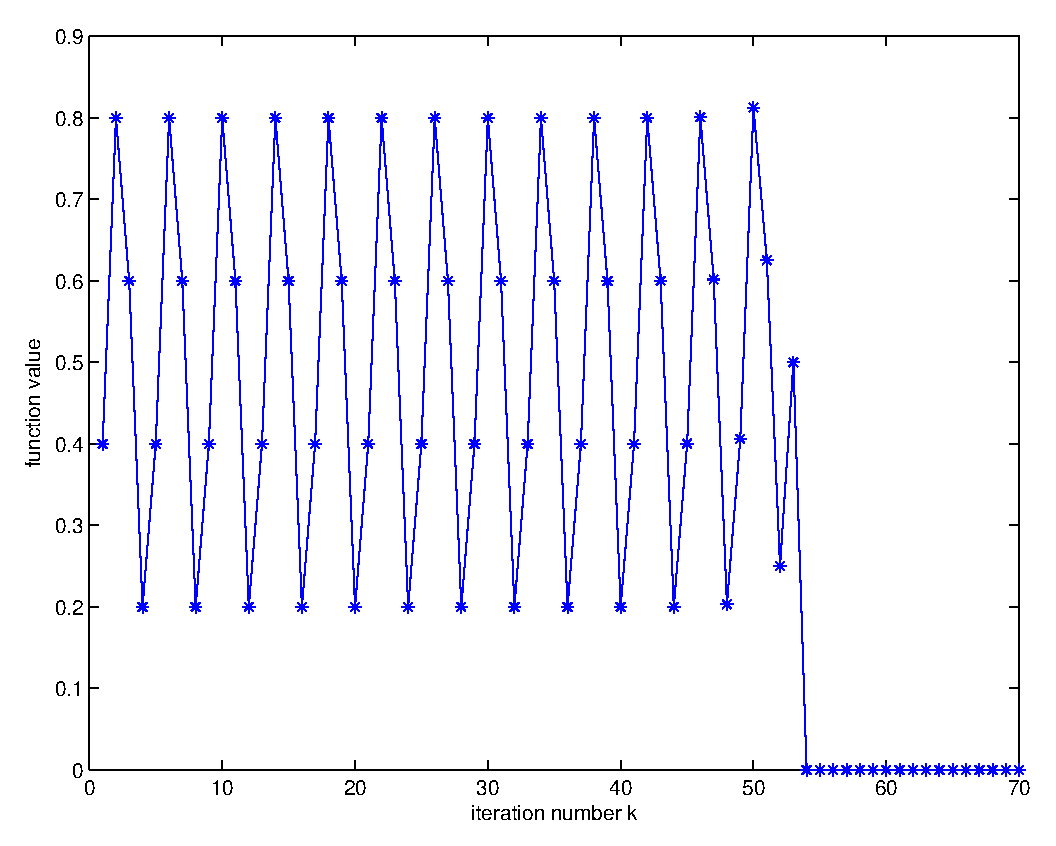
\includegraphics[width=0.4\textwidth]{doubling.eps}\\
  \caption{一个简单的例子, 表明舍入误差可能对一个算法造成很大的影响.}
  \label{fig:doubling}
\end{figure}

实际上, 关于为什么不带最小二乘的几何构建算法算不好大规模的精确距离的问题 
(尽管理论上很完美),
这个例子也可以给我们一些洞见, 误差累积是这个迭代算法一个很重要的因素.
在带误差的情形中, 距离误差带来的定位的不精确比累积误差大得多,
这会对迭代计算产生更大的影响. 
从这里也可以看出为什么带大的距离噪音的距离几何问题如此困难.


